\documentclass{lehramt-informatik-aufgabe}
\liLadePakete{gantt,cpm}
\begin{document}
\liAufgabenMetadaten{
  Titel = {Aufgabe 2},
  Thematik = {Projektplanung},
  RelativerPfad = Staatsexamen/66116/2020/09/Thema-1/Teilaufgabe-1/Aufgabe-2.tex,
  ZitatSchluessel = examen:66116:2020:09,
  BearbeitungsStand = unbekannt,
  Korrektheit = unbekannt,
  Stichwoerter = {Projektplanung, CPM-Netzplantechnik, Gantt-Diagramm},
  ExamenNummer = 66116,
  ExamenJahr = 2020,
  ExamenMonat = 09,
  ExamenThemaNr = 1,
  ExamenTeilaufgabeNr = 1,
  ExamenAufgabeNr = 2,
}

\let\f=\footnotesize
\let\FZ=\liCpmFruehesterI
\let\SZ=\liCpmSpaetesterI
\let\v=\liCpmVon
\let\vz=\liCpmVonZu
\let\z=\liCpmZu

Die Planung eines Softwareprojekts kann \zB in Form von
Gantt-Diagrammen oder CPM-Netzwerken (kritischer Pfad Methode)
festgehalten werden.

Folgendes Gantt-Diagramm zeigt einen Teil der Projektplanung in einem
klassischen Softwareentwicklungsprozess:
\index{Projektplanung}
\footcite{examen:66116:2020:09}

\begin{center}
\begin{ganttchart}[x unit=0.7cm, y unit chart=0.6cm]{0}{6}
\ganttbar[name=D]{Design}{0}{1} \\
\ganttbar[name=R]{Realization}{2}{4} \\
\ganttbar[name=T]{Testing}{3}{5}
\gantttitlelist[name=Zeit]{0,...,6}{1}\\
\ganttlink{D}{R}
\ganttlink[link type=s-s]{R}{T}
\end{ganttchart}
\end{center}
\begin{enumerate}

%%
% (a)
%%

\item Im Diagramm werden 3 Phasen aus dem klassischen
Softwareentwicklungsprozess genannt. Welche Phase sollte dem Design
(Entwurf) immer vorangehen?

\begin{liAntwort}
Die Anforderungsdefinition
\end{liAntwort}

%%
% (b)
%%

\item Wandeln Sie das Gantt-Diagramm in ein CPM-Netzwerk um. Fügen Sie
dazu einen zusätzlichen Start- und Endknoten hinzu. Das Ende des
Projekts ist durch das Ende aller Aktivitäten bedingt.
\index{CPM-Netzplantechnik}

\begin{liAntwort}
\begin{description}
\item[$D_A$] Design Anfang
\item[$R_A$] Realization Anfang
\item[$T_A$] Testing Anfang
\item[$D_E$] Design Ende
\item[$R_E$] Realization Ende
\item[$T_E$] Testing Ende

\end{description}

\begin{center}
\begin{tikzpicture}[x=1.5cm,y=1.5cm]
\liCpmEreignis[name=A]{$A$}{1}{1}
\liCpmEreignis[name=DA]{$D_A$}{1}{2}
\liCpmEreignis[name=DE]{$D_E$}{3}{2}
\liCpmEreignis[name=RA]{$R_A$}{2}{1}
\liCpmEreignis[name=RE]{$R_E$}{4}{1}
\liCpmEreignis[name=TA]{$T_A$}{3}{0}
\liCpmEreignis[name=TE]{$T_E$}{5}{0}
\liCpmEreignis[name=E]{$E$}{5}{1}

\liCpmVorgang[schein]{A}{DA}{}
\liCpmVorgang{DA}{DE}{2}
\liCpmVorgang{RA}{RE}{3}
\liCpmVorgang{TA}{TE}{3}
\liCpmVorgang{RA}{TA}{1}
\liCpmVorgang[schein]{DE}{RA}{}
\liCpmVorgang[schein]{TE}{E}{}
\liCpmVorgang[schein]{RE}{E}{}
\end{tikzpicture}
\end{center}
\end{liAntwort}
%%
% (c)
%%

\item Welche im obigen Gantt-Diagramm nicht enthaltenen Beziehungsarten
zwischen Aktivitäten können in einem Gantt-Diagramm noch auftreten?
Nennen Sie auch deren Bedeutung.
\index{Gantt-Diagramm}

\begin{liAntwort}
Diese Beziehungsarten sind im obigen Gantt-Diagramm vorhanden:

\begin{description}
\item[Normalfolge EA:]
\emph{end-to-start relationship}
%
Anordnungsbeziehung vom Ende eines Vorgangs zum Anfang seines
Nachfolgers.

\item[Anfangsfolge AA:]
\emph{start-to-start relationship}
%
Anordnungsbeziehung vom Anfang eines Vorgangs zum Anfang seines
Nachfolgers.
\end{description}

Diese Beziehungsarten sind im obigen Gantt-Diagramm \emph{nicht}
vorhanden:
\begin{description}

\item[Endefolge EE:]
\emph{finish-to-finish relationship}
%
Anordnungsbeziehung vom Ende eines Vorgangs zum Ende seines Nachfolgers.

\item[Sprungfolge AE:]
\emph{start-to-finish relationship }
%
Anordnungsbeziehung vom Anfang eines Vorgangs zum Ende seines
Nachfolgers
\end{description}
\end{liAntwort}

Gegeben sei nun das folgende CPM-Netzwerk:

\begin{center}
\begin{tikzpicture}[x=1.5cm,y=1.5cm]
\liCpmEreignis{a}{0}{1}
\liCpmEreignis{b}{1}{2}
\liCpmEreignis{c}{2}{2}
\liCpmEreignis{d}{2}{1}
\liCpmEreignis{e}{3}{1}
\liCpmEreignis{f}{2}{0}
\liCpmEreignis{g}{4}{1}

\liCpmVorgang[schein]{b}{d}{}
\liCpmVorgang[schein]{b}{f}{}
\liCpmVorgang[schein]{d}{e}{}
\liCpmVorgang{a}{b}{2}
\liCpmVorgang{a}{f}{3}
\liCpmVorgang{b}{c}{3}
\liCpmVorgang{c}{d}{1}
\liCpmVorgang{c}{e}{5}
\liCpmVorgang{e}{g}{2}
\liCpmVorgang{f}{e}{4}
\end{tikzpicture}
\end{center}

%%
% (d)
%%

\item Geben Sie für jedes Ereignis die früheste Zeit an.

\begin{liAntwort}
\begin{tabular}{|l|r|r|}
$i$ & Nebenrechnung & \FZ \\\hline\hline
a &                        & 0 \\
b &                        & 2 \\
c &                        & 5 \\
d & $\max(2_b, 6_c)$       & 6 \\
e & $\max(6_d, 10_e, 7_f)$ & 10 \\
f & $\max(3_f, 2_b)$       & 3 \\
g &                        & 12 \\
\end{tabular}
\end{liAntwort}

%%
% (e)
%%

\item Geben Sie für jedes Ereignis die späteste Zeit an.

\begin{liAntwort}
\begin{tabular}{|l|r|r|}
$i$ & Nebenrechnung & \SZ \\\hline\hline
a &                        & 0 \\
b & $\min(2_c, 10_d, 6_f)$ & 2 \\
c & $\min(9_d, 5_e)$       & 5 \\
d &                        & 10 \\
e &                        & 10 \\
f &                        & 6 \\
g &                        & 12 \\
\end{tabular}
\end{liAntwort}

%%
% (f)
%%

\item Geben Sie einen kritischen Pfad durch das Netz an! Wie wirkt sich
eine Verzögerung von 5 Zeiteinheiten auf dem kritischen Pfad auf das
Projektende aus?

\begin{liAntwort}
\begin{tabular}{|l|l|l|l|l|l|l|l|}
\hline
$i$ & a & b & c  & d  & e  & f  & g  \\\hline\hline
\FZ & 0 & 2 & 5  & 6  & 10 & 3  & 12 \\\hline
\SZ & 0 & 2 & 5  & 10 & 10 & 6  & 12 \\\hline
GP  & 0 & 0 & 0  & 3  & 0  & 3  & 0  \\\hline
\end{tabular}

\begin{center}
\begin{tikzpicture}[x=1.5cm,y=1.5cm]
\liCpmEreignis{a}{0}{1}
\liCpmEreignis{b}{1}{2}
\liCpmEreignis{c}{2}{2}
\liCpmEreignis{d}{2}{1}
\liCpmEreignis{e}{3}{1}
\liCpmEreignis{f}{2}{0}
\liCpmEreignis{g}{4}{1}

\liCpmVorgang[schein]{b}{d}{}
\liCpmVorgang[schein]{b}{f}{}
\liCpmVorgang[schein]{d}{e}{}
\liCpmVorgang[kritisch]{a}{b}{2}
\liCpmVorgang{a}{f}{3}
\liCpmVorgang[kritisch]{b}{c}{3}
\liCpmVorgang{c}{d}{1}
\liCpmVorgang[kritisch]{c}{e}{5}
\liCpmVorgang[kritisch]{e}{g}{2}
\liCpmVorgang{f}{e}{4}
\end{tikzpicture}
\end{center}

Kritischer Pfad: a $\rightarrow$ b $\rightarrow$ c $\rightarrow$ e $\rightarrow$ g

Das Projekt verlängert sich um 5 Zeiteinheiten.
\end{liAntwort}

\end{enumerate}
\end{document}
